\documentclass[a4paper,14pt]{extarticle}
% Преамбула создана для онлайн-смены "Абитуриент 2022"
% Автор - Баринов Леонид, telegram: @leonidka2001
%
% pdflatex
%
% Кодировка. Существуюет входная и внутренняя кодировка.
% Мы будем пользоваться внутренней кодировкой T2A и входной
% кодировкой utf8. Стоит понимать, что это большой костыль!
% Если создаете новые собственные файлы используйте другие 
% версия TeXa, которые хорошо работают с разными языками и
% различными математическими шрифтами, например, xelatex!
\usepackage[T2A]{fontenc}
\usepackage[utf8]{inputenc}


% Для соблюдения типографских традиций и возможности переноса
% слов в различных языках нужен пакет babel. Языки указывается через запятую,
% основный язык документа указывается последним

\usepackage[english,russian]{babel}


%-----------------------------------------------------
%% xelatex
%
%% Если используете xelatex, переключите компилятор на xelatex
%% закомментируйте строчки с fontenc, inputenc, babel и amssymb
%% раскомментируйте строчки ниже до следующей линии ----
%
%% Вместо babel
%\usepackage{polyglossia}   
%\setdefaultlanguage{russian}  
%\setotherlanguage{english} 
%
%% Подключение математических символов
%\usepackage{unicode-math}
%
%\setmainfont{CMU Serif} %% задаёт основной шрифт документа
%\setsansfont{CMU Sans Serif} %% задаёт шрифт без засечек
%\setmonofont{CMU Typewriter Text} %% задаёт моноширинный шрифт
%\setmathfont{latinmodern-math.otf}
%\setmathfont[range={\rightarrow,\leftarrow,\int,\vartriangle, \mitg}]{XITS Math}
%
%% Возможность использования русских букв в математическом
%% режиме без команды \text{text}
%
%\DeclareSymbolFont{cyrletters}{\encodingdefault}{\familydefault}{m}{}
%\newcommand{\makecyrmathletter}[1]{%
	%	\begingroup\lccode`a=#1\lowercase{\endgroup
		%		\Umathcode`a}="0 \csname symcyrletters\endcsname\space #1
	%}
%\count255="409
%\loop\ifnum\count255<"44F
%\advance\count255 by 1
%\makecyrmathletter{\count255}
%\repeat

%------------------------------------------------------

% Работа с математическими символами, добавление
% различных математических окружений.
% Спасибо Американскому математическому обществу!

\usepackage{amsmath,amsfonts,amsthm, mathtools}
\usepackage{amssymb}

% Вставка рисунков. Можно указать место, где необходимо
% искать изображения

\usepackage{graphicx}
\graphicspath{{images/}}

% Вставка плавающих объектов (занимающих часть страницы)
\usepackage{wrapfig}

% latex вставляет рисунки по определенному алгоритму. Его,
% конечно, можно менять, но это не настолько просто. Как
% правило, хочется, чтобы картинка располагалась там, где мы это
% указали в коде. Для этого существует несколько пакетов, один из
% них floatrow. Он позволяет для окружения figure указывать
% необязательный аргумент - H (именно большое h), что на latex'овском
% языке означает: вставить картинку здесь и только здесь. (даже если
% облик документа несколько пострадает)

\usepackage{floatrow}

% По правилам оформления рисунок всегда должен быть подписан. Для
% этого существует команда \caption{}. Но обычные настройки caption
% оставлять желать лучшего. Хотелось сделать подпись меньше
% основного шрифта, а также слово Рис жирным и использовать
% разделитель точку, а не двоеточие. В этом помогает пакет,
% который называется caption (совпадение?)

\usepackage{setspace}
\usepackage[margin=10pt,font={small,stretch=0.9},labelfont=bf,labelsep=period,
justification=centerlast]{caption}

% Оформление и создание таблиц 

\usepackage{array,tabularx,tabulary,booktabs}

% Великолепный новый пакет для работы с таблицами
% \usepackage{tabularray}

% После excel есть ощущения, что везде объединить колонки или строки
% легко. В latex не совсем так. Помогают пакеты multirow, multicol. 

\RequirePackage{multirow}
\RequirePackage{multicol}

% Иногда могут потребоваться длинные таблицы на несколько страниц.
% Обычные таблицы latex воспринимает как одну букву. И
% становиться понятно, почему возникают проблемы при переносе
% обычной таблицы. (Ведь нельзя же перенести одну букву!). Поэтому
% вместо обычной таблицы нужна длинная таблица.

\RequirePackage{longtable}

% В русской типографской традиции принято начинать каждый новый абзац
% с красной строки. Даже первый после заголовка (или подзаголовка).
% Чтобы каждый раз не ставить красную строку вручную существует пакет
% indentfirst

\usepackage{indentfirst}


% Работа со ссыллаками:
\usepackage{hyperref}

% Целая дробная часть у нас разделяется запятой,
% однако так принято не во всём мире. Чтобы TeX
% воспринимал запятую как разделитель целой и дробной
% части необходим пакет icomma

\usepackage{icomma}

%% Перенос знаков в формулах (по Львовскому)
\newcommand*{\hm}[1]{#1\nobreak\discretionary{}
	{\hbox{$\mathsurround=0pt #1$}}{}}

% Модификаторы начертания
\usepackage{soulutf8} 

%%% Программирование
\usepackage{etoolbox} % логические операторы

% Работа с колонтитулами
\usepackage{fancyhdr}
%\pagestyle{fancy}
\renewcommand{\headrulewidth}{0mm} % Если необходимо убрать линейку, или изменить ее длину
% \lfoot{\thepage} % Нижний левый
\cfoot{\thepage} % Нижний в центре
% \rfoot{} % Нижний правый
% \rhead{} % Верхний правый
% \chead{} % Верхний в центре
% \lhead{} % Верхний левый



% Задание полей документа. Есть несколько способов, но
% самый простой из них - это воспользоваться пакетом geometry, который
% позволяет определить все поля документа (начиная с краев листа, что
% важно, так как некоторые другие способы позволяют это сделать только косвенно)

\usepackage{geometry}
\geometry{top=20mm}
\geometry{bottom=20mm}
\geometry{left=20mm}
\geometry{right=20mm}

% Свои команды
\DeclareMathOperator{\sgn}{\mathop{sgn}}



\begin{document}
	
	\begin{center}
		\textit{Федеральное государственное автономное образовательное\\ учреждение высшего образования }
		
		\vspace{0.5ex}
		
		\textbf{«Московский физико-технический институт\\ (национальный исследовательский университет)»}
	\end{center}
	
	\vspace{10ex}
	
	
	\begin{center}
		\vspace{13ex}
		
		\textbf{Лабораторная работа №1.2.1}
		
		\vspace{1ex}
		
		по курсу общей физики
		
		на тему:
		
		\textbf{\textit{<<Определение скорости полета пули при помощи баллистического маятника (1.2.1)>>}}
		
		\vspace{30ex}
		
		\begin{flushright}
			\noindent
			\textit{Работу выполнил:}\\  
			\textit{Третьяков Александр \\(группа Б02-206)}
		\end{flushright}
		\vfill
		Долгопрудный \\ \today
		
		%\setcounter{page}{1}


	
	\section{Введение}
	
	\textbf{Цель работы:}
	Определить скорость полёта пули применяя законы сохранения и использую баллистические маятники
	
	\noindent\textbf{Оборудование:}
	Духовое ружьё на штативе, осветитель, оптическая система для измерения отклонений маятника, измерительная линейка, пули и весы для их взвешивания, баллистические маятники.
	\section{Ход работы}
	
	\subsection{Метод баллистического маятника, совершающего поступательное движение}
	В этой части работы будем использовать установку, изображённую на рисунке ниже. При попадании пули в цилиндр любая его точка движется по окружности известного радиуса, поэтому его смещение с помощью собирающей линзы можно перевести в линейное отклонение на линейке.
	
	\begin{figure}[H]
		\begin{center}
			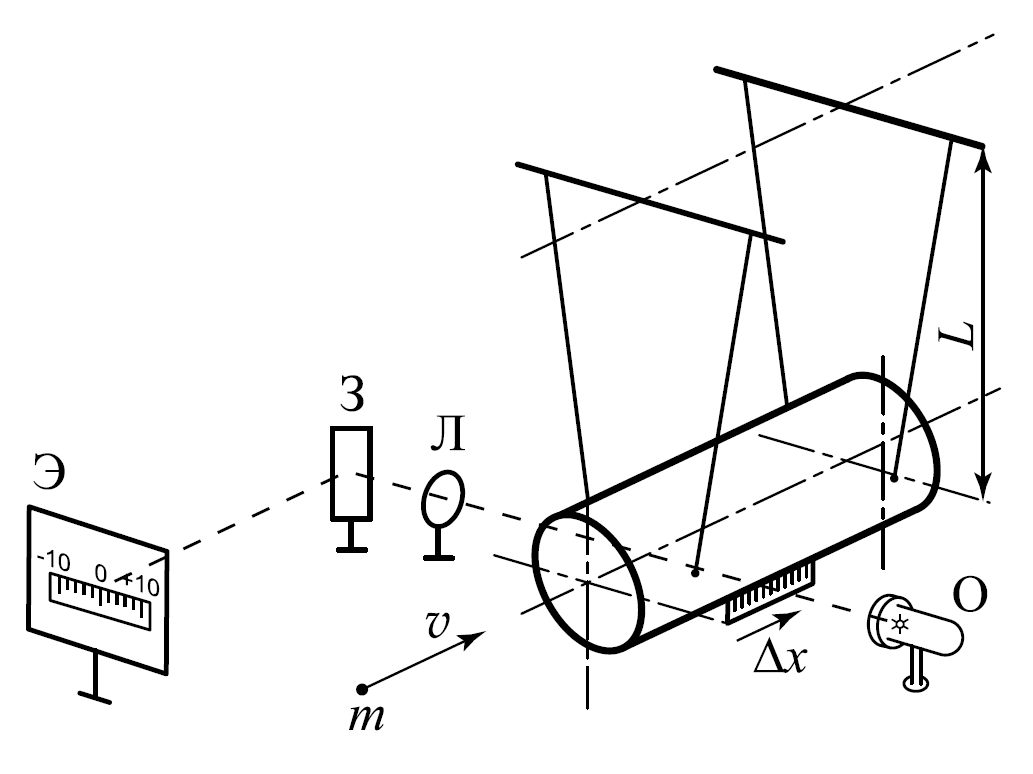
\includegraphics[scale = 0.56]{1.2.1 ustan1}
			\caption{схема установки для измерения скорости полета пули}
		\end{center}
	\end{figure}
	
	При контакте пули с цилиндром можно записать ЗСИ:
	\begin{equation}
		mu = (M+m)V
	\end{equation}
	где $m$ -- масса пули, $u$ -- скорость пули перед ударом, $V$-скорость цилиндра вместе с пулей после удара.
	\begin{equation}
		u=\frac{M+m}{m}V \approx \frac{M}{m}V \;\;\;\;\; V^2=2gh \;\;\;\;\; h = L(1-cos \varphi ) = 2L^2 sin \frac{\varphi^2}{2} \;\;\;\;\;\;\; \varphi \approx \frac{\Delta x}{L} 
	\end{equation}
	Тогда скорость пули можно выразить как
	\begin{equation} \label{vel1}
		u=\frac{M}{m} \sqrt{\frac{g}{L}} \Delta x
	\end{equation}
	
	При измерении было замечено, что за 10 периодов амплитуда колебаний почти не уменьшилась, поэтому их затуханием можно пренебречь.
	
	Для начала проверим работоспособность установки, а именно проведем несколько холостых выстрелов по маятнику и убедимся в том, что он практически не реагирует на удар воздушной струи.
	
	Вычислять скорость пули будем по форуле \eqref{vel1}, для чего нужно проверить, что за 10 колебаний амплитуда уменьшалается меньше, чем на половину.
	
	Произведем 4 выстрела, запишем амплитуды, полученные при выстрелах, и по их значениям найдем скорости пуль.
	

	
	\noindent наша установка имела параметры: $M = (2925 \pm 5)$ г, и $L = (220,4 \pm 0,1)$ см.
	
	Средняя скорость пули \underline{$u_\text{ср} = 163,9$ м/с}, а погрешность будет равна:
	
	\begin{equation}
		\sigma_u^{\text{сист}} =u \sqrt{\varepsilon_M^2 + \varepsilon_m^2 + \varepsilon_{\Delta x}^2 + \left(\frac{\varepsilon_L}{2} \right)^2}  \;\;\;\;\; \sigma_u^{\text{случ}} = \sqrt{ \frac{1}{n(n-1)} \sum_{i=1}^{n}(u_i - u_{\text{ср}})^2} \;\;\;\;\; \sigma_u =\sqrt{\sigma_{\text{сист}}^2 + \sigma_\text{случ}^2} 
	\end{equation}
	\begin{equation}
		\sigma_u^\text{сист}\approx 3,1 \text{ }\dfrac{\text{м}}{\text{с}} \;\;\;\;\;\;\;\;\;\;\;\;\;\;\;\;\;\;\;\;\;\;\;\;\;\;\;\;\;\;\; \sigma_u^\text{случ}\approx 2,9 \text{ }\dfrac{\text{м}}{\text{с}} \;\;\;\;\;\;\;\;\;\;\;\;\;\;\;\;\;\;\;\;\;\;\;\;\;\;\;\;\;\;\;
		\sigma_u \approx 4,2 \text{ }\dfrac{\text{м}}{\text{с}}
	\end{equation}
	
	Окончательно получаем скорость пули равную \underline{$u = (163,9 \pm 4,2)\text{, }\dfrac{\text{м}}{\text{с}}$}
	
	\subsection{Метод крутильного баллистического маятника}
	
	В этой части работы мы будем использовать крутильный баллистический маятник. Схема установки представлена на картинке ниже.
	
	\begin{figure}[h]
		\begin{center}
			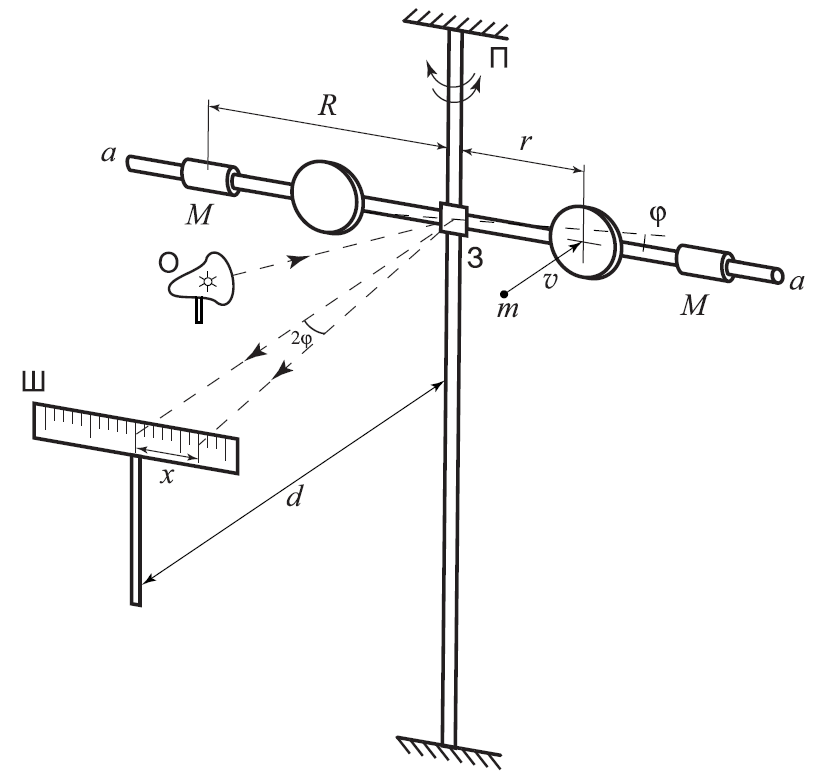
\includegraphics[scale = 0.66]{1.2.1 ustan2}
			\caption{схема установки для измерения скорости полета пули с баллистическим маятником}
		\end{center}
	\end{figure}
	
	Считая удар неупругим, можно записать уравнение
	$$mur=I \Omega$$
	$r-$расстояние от линии полёта пули до оси вращения, $I$ -- момент инерции относительно этой оси, $\Omega$ -- угловая скорость маятника сразу после удара.
	
	Можно пренебречь затуханием колебаний и потерями энергии и записать ЗСЭ:
	$$ k \frac{\varphi^2}{2} = I \frac{\Omega^2}{2} $$
	\noindent где $k$ -- модуль кручения проволоки, $\varphi$ -- максимальный угол поворота маятника, тогда:
	\begin{equation} \label{vel2}
		u = \varphi \frac{\sqrt{kI}}{mr} 
	\end{equation}
	Измерим растояние от оси вращения до штатива с линейкой $d = 59,3 \pm 0,1 \text{ см}$, тогда в силу малости колебаний можно найти $\varphi$ как
	
	\begin{equation}
		\label{phi}
		\varphi \approx \frac{x}{2d}
	\end{equation}
	
	где $x$ -- смещение изображения нити осветителя на шкале, которое легко можно измерить.
	
	Периоды колебаний маятника с грузами и без можно выразить как
	$$T_1= 2 \pi \sqrt{\frac{I - 2MR^2}{k}} \;\;\;\;\;\; T_2 = 2 \pi \sqrt{\frac{I}{k}}$$
	Тогда $\sqrt{kI}$ можно найти как:
	\begin{equation}
		\sqrt{kI} = \frac{4 \pi M R^2 T_2}{T_2^2 - T_1^2}
		\label{kl}
	\end{equation}
	$R$ -- расстояние от оси вращения до центров грузиков, $M$ - масса грузиков.
	
	Для начала запишем данные установки: $ r = 22 \text{ см} \text{, } R = 33,6 \text{ см} \text{, } M_1 = 729,9\text{ г} \text{, а } M_2 = 729,6 \text{ г} $.
	
	Снимем периоды колебаний после выстрела с грузиками и без, чтобы найти $\sqrt{kI}$:
	

	
	Из таблицы получаем, что $T_1^{\text{ср}} = (15,387 \pm 0,207) \text{ см}$, а $T_2^{\text{ср}} = (19,946 \pm 0,03)\text{ см}$. С помощью полученных периодов колебаний найдем $\sqrt{kI}$ по формуле \eqref{kl}:
	
	$$\sqrt{kI} \approx 138,18 \cdot 10^{-3} \text{ } \dfrac{\text{кг}\cdot\text{м}^2}{\text{c}} \;\;\;\;\;\; \sigma_{\sqrt{kI}} = \sqrt{kI} \cdot \sqrt{\varepsilon_{T_2^2-T_1^2}^2 + \left(2\varepsilon_{R^2}\right)^2 + \varepsilon_M^2 + \varepsilon_{T^2}^2} \approx 0,54 \cdot 10^{-3} \text{ } \dfrac{\text{кг}\cdot\text{м}^2}{\text{c}}$$
	
	Теперь по формулам \eqref{vel2} и \eqref{phi} определим $\varphi$ и скорость пули. Получаем таблицу:
	
	\begin{equation}
		\sigma_u^{\text{сист}} = u\cdot \sqrt{ \varepsilon_x^2+ \varepsilon_d^2+ \varepsilon_{\sqrt{kI}}^2 + \varepsilon_m^2 + \varepsilon_r^2 } \;\;\;\;\;\; \sigma_u^{\text{случ}} =  \sqrt{\frac{1}{n(n-1)} \sum_{i=1}^{n}(u_i - \overline{u})^2} \;\;\;\;\;\;
		\sigma_u = \sqrt{\sigma_{\text{случ}}^2 + \sigma_\text{сист}^2}
	\end{equation}
	
	Тогда средняя скорость \underline{$u_\text{ср} = (159,95 \pm 1,44)\text{ }\frac{\text{м}}{\text{с}} $}
	
	\section{Вывод}
	
	\indent Были полученны скорости пули двумя методами:  методом баллистического маятника, совершающего поступательное движение, и методом крутильного баллистического маятника. Разброс полученных значений связан как с ошибками опыта, так и с различием скоростей пуль от выстрела к выстрелу. Так же имеет значение то, что стрельба в каждом методе производилась своим ружьем.
	

\end{document}